\documentclass[t,compress,10pt,xcolor=dvipsnames]{beamer}

\usepackage{lmodern}
\usepackage[labelformat=empty,labelsep=none]{subfig}
\usepackage{caption}
\usepackage{float}
\usepackage{wrapfig}

\newcommand*\oldmacro{}%
\let\oldmacro\insertshorttitle% 
\renewcommand*\insertshorttitle{%
\oldmacro\hfill%
\insertframenumber\,/\,\inserttotalframenumber}

\definecolor{UniDunkel}{RGB}{73,142,137}
\definecolor{UniHell}{RGB}{142,184,182}

\setbeamertemplate{blocks}[rounded][shadow=true]
\setbeamercolor{structure}{fg=UniDunkel}

\setbeamercolor{block body}{parent=normal text,use=block title,bg=block title.bg!10!bg}
\setbeamercolor{block body alerted}{parent=normal text,use=block title alerted,bg=block title alerted.bg!10!bg}
\setbeamercolor{block body example}{parent=normal text,use=block title example,bg=block title example.bg!10!bg}

\setbeamercolor*{palette primary}{use=structure,fg=white,bg=UniDunkel!115}
\setbeamercolor*{palette secondary}{use=structure, fg=UniHell,  bg=UniHell}
\setbeamercolor*{palette tertiary}{use=structure,fg=white,bg=UniDunkel!115}
\setbeamercolor*{palette quaternary}{fg=Orange}

\setbeamercolor*{sidebar}{use=structure,bg=structure.fg}
\setbeamercolor*{palette sidebar primary}{use=structure,fg=structure.fg!10}
\setbeamercolor*{palette sidebar secondary}{fg=white}
\setbeamercolor*{palette sidebar quaternary}{fg=white}
\setbeamercolor*{titlelike}{parent=palette primary}

\setbeamercolor*{fine separation line}{}

\setbeamercolor{block title}{use=structure,fg=white,bg=structure.fg!0!red}
\setbeamercolor{block title alerted}{use=alerted text,fg=white,bg=alerted text.fg!0!white}
\setbeamercolor{block title example}{use=example text,fg=white,bg=example text.fg!0!white}

\useoutertheme{miniframes}
\useinnertheme{circles}
\setbeamertemplate{footline}[frame number]

\beamertemplatenavigationsymbolsempty

\usepackage{textpos} 
\usepackage{mathptmx}
\usepackage{anyfontsize}
\usepackage{t1enc}
\usepackage{multicol}
\usepackage{lmodern}

%\addtobeamertemplate{frametitle}{}{%
%\begin{textblock*}{100mm}(11cm,-1cm)
%	\includegraphics[height=1cm]{logo.png}
%\end{textblock*}}

%\titlegraphic{
%	\includegraphics[width=5cm]{backg}
%}

\title{\textbf{Agrupamiento y clasificaci\'on en la recuperaci\'on de informaci\'on en la web}}

%\author{Integrantes:\\
%	Marcos Manuel Tirador del Riego\\ 
%	Laura Victoria Riera P\'erez\\
%	Leandro Rodr\'iguez Llosa}
%\institute{Ciencias de la computaci\'on}
\date{}

%\usepackage{tikz}
%\titlegraphic { 
%	\begin{tikzpicture}[remember picture]
%		\node[left=0.2cm] at (current page.30){
%			\includegraphics[width=10cm]{backg}
%		};
%	\end{tikzpicture}
%}

\setbeamercolor{block body}{bg=Emerald,fg=Emerald}



\begin{document}
	
	\begin{frame}
		\begin{center}
			\begin{block}{}
				\centering
				\Large\textcolor{white}{\textbf{Agrupamiento y clasificaci\'on en la recuperaci\'on de informaci\'on en la web}}
			\end{block}
		
		\vspace{0.5em}
		
\includegraphics[width=3cm]{clustering.jpg}
		
		\vspace{0.5em}
		\footnotesize
		Integrantes:\\
			Marcos Manuel Tirador del Riego\\ 
			Laura Victoria Riera P\'erez
		
		\vspace{0.7em}
		\tiny	
		Tercer año. Ciencias de la computaci\'on. Universidad de La Habana. Cuba.
		
		\vspace{0.7em}
		\scriptsize
		Noviembre, 2022
		\end{center}
	\end{frame}

	\begin{frame}[allowframebreaks]{\'Indice general}
		\tableofcontents[sections={1}]
		\framebreak
		\tableofcontents[sections={2-4}]
	\end{frame}

	\frame{
		\frametitle{Aprendizaje no supervisado vs. aprendizaje supervisado}
		\begin{center}
			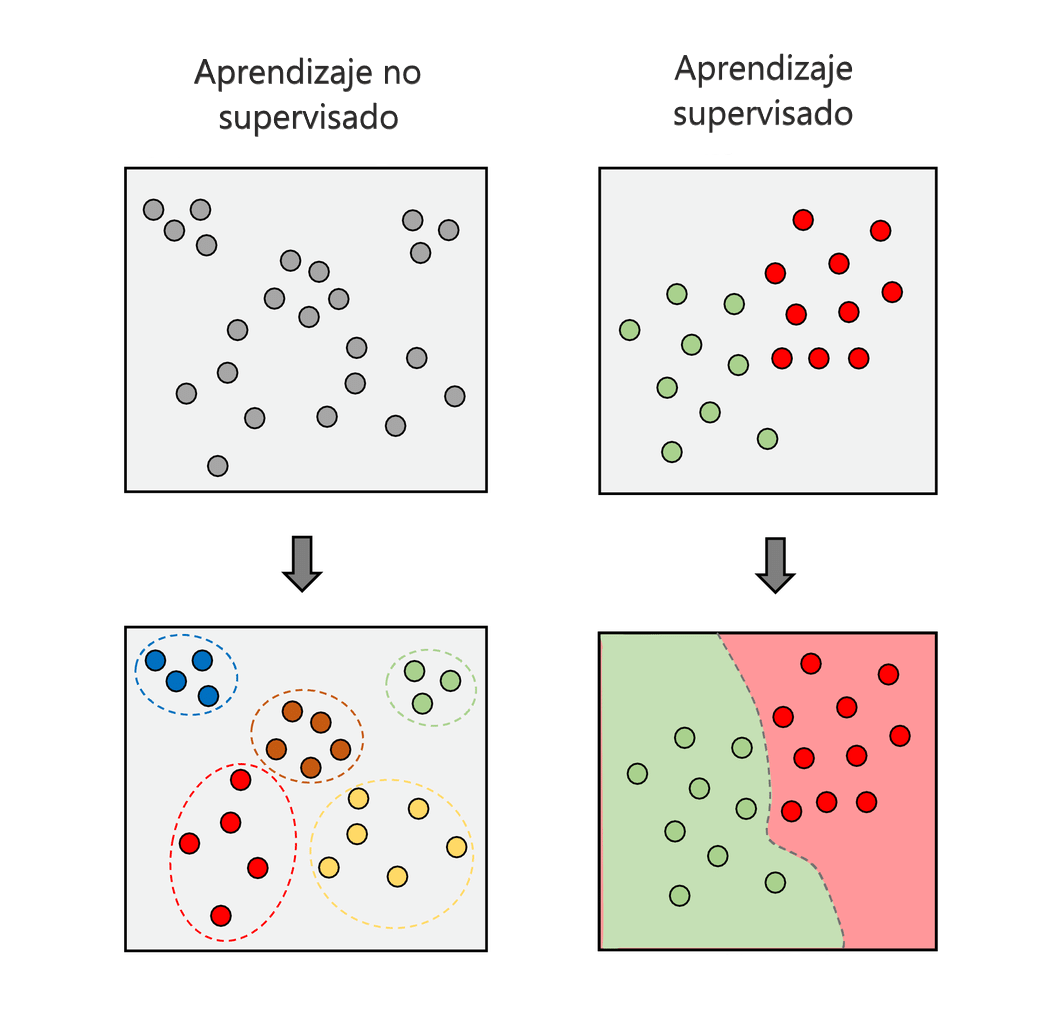
\includegraphics[width=7cm]{UL_vs_SL.png}
		\end{center}
	}
	\section{Agrupamiento}
	\frame[allowframebreaks]
	{
		\frametitle{Agrupamiento}
		\vspace{1em}
		Los algoritmos de agrupamiento conglomeran un conjunto de documentos en subconjuntos o clústeres. Son utilizados para generar una estructura de categorías que se ajuste a un conjunto de observaciones. 
		
	\begin{center}
		\vspace{0.5em}
		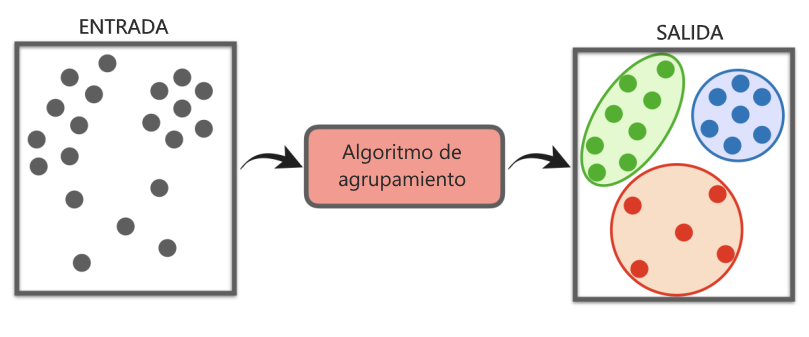
\includegraphics[width=10cm]{clustering_notion1.png}
	\end{center}
	}

	\frame{
		\frametitle{Caracter\'isticas generales}
		
		\vspace{4em}
		\begin{itemize}
			\item Es la forma más común de aprendizaje no supervisado.
			\item Los grupos formados deben tener un alto grado de asociación entre los documentos de un mismo grupo y un bajo grado entre miembros de diferentes grupos.
			\item La entrada clave para un algoritmo de agrupamiento es la medida de distancia. Diferentes medidas de distancia dan lugar a diferentes agrupamientos. 
		\end{itemize}
	}
	
	\frame{
		\frametitle{Hip\'otesis de agrupamiento}
		
		\vspace{5em}
		\textit{"Los documentos en el mismo grupo se comportan de manera similar con respecto a la relevancia para las necesidades de información."}
		
		\vspace{2em}
		La hipótesis establece que si hay un documento de un grupo que es relevante a una solicitud de búsqueda, entonces es probable que otros documentos del mismo clúster también sean relevantes. 
	}

	\frame{
		\frametitle{Clasificaci\'on de los algoritmos de agrupamiento}
		
		\vspace{2.5em}
		Seg\'un la pertenencia a los grupos:
		\begin{itemize}
			\item \textit{agrupamiento exclusivo o fuerte} (hard clustering): cada documento es miembro de exactamente un grupo.
			\item \textit{agrupamiento difuso o suave} (soft clustering): un documento tiene membresía fraccionaria en varios grupos.
		\end{itemize}
		
		\vspace{2em}
		Seg\'un el tipo de estructura impuesta sobre los datos:
		\begin{itemize}
			\item \textit{agrupamiento particionado o plano} (flat clustering)
			\item \textit{agrupamiento difuso o suave} (soft clustering): \textit{agrupamiento jer\'arquico} (hierarchical clustering).
		\end{itemize}
	}

	\subsection{Medidas de similitud entre documentos}
	\frame{
		\frametitle{Medidas de similitud}
		Sean $ d_{i} $ el documento $ i $ del corpus y $ w_{ik} $ el peso del t\'ermino $ k $ de un total $ N $ ($ N > 0 $) en el documento $ i $ .
		
		\begin{itemize}
			\vspace{0.5em}
			\item \textbf{Coeficiente de Dice:}
			\begin{center}
				$ S_{d_{i}, d_{j}} = \dfrac{2 \sum_{k=1}^{N} (w_{ik}w_{jk})}{\sum_{k=1}^{N}w_{ik}^{2} + \sum_{k=1}^{N}w_{jk}^{2}} $
			\end{center}
			
			\vspace{0.5em}
			\item \textbf{Coeficiente de Jaccard:}
			\begin{center}
				$ S_{d_{i}, d_{j}} = \dfrac{\sum_{k=1}^{N} (w_{ik}w_{jk})}{\sum_{k=1}^{N}w_{ik}^{2} + \sum_{k=1}^{max}w_{jk}^{2} - \sum_{k=1}^{N} (w_{ik}w_{jk})} $
			\end{center}
		
			\vspace{0.5em}
			\item \textbf{Coeficiente del coseno:}
			\begin{center}
				$ S_{d_{i}, d_{j}} = \dfrac{\sum_{k=1}^{N} (w_{ik}w_{jk})}{\sqrt{\sum_{k=1}^{N}w_{ik}^{2} \sum_{k=1}^{N}w_{jk}^{2}}} $
			\end{center}
		\end{itemize}
	
	}
	
	\subsection{Medidas de evaluaci\'on}
	\frame[allowframebreaks]
	{
		\frametitle{Medidas de evaluaci\'on}
		\begin{itemize}
			\vspace{0.5em}
			\item \textbf{Pureza:} Para calcular la pureza, cada grupo se asigna a la clase que es más frecuente en el grupo, y luego se mide la precisión de esta asignación contando el número de documentos correctamente asignados y dividiendo por N.
			
			\vspace{0.5em}
			\begin{center}
				$purity(\Omega, C) = \dfrac{1}{N} \sum_{k}max_{j} |\omega_{k} \cap c_{j}| $
			\end{center}
			\vspace{0.5em}
			
			donde:
			\begin{itemize}
				\item $ \Omega = \{\omega_{1}, \omega_{2}, ... , \omega_{K}\} $ $\rightarrow$ conjunto de cl\'usters
				\item $ C = \{c_{1}, c_{2}, ... , c_{J}\} $ $\rightarrow$ conjunto de clases
			\end{itemize}
			
			\vspace{0.5em}
			Se interpreta $ \omega_{k} $ como el conjunto de documentos en el cl\'uster y $ c_{j} $ como el conjunto de documentos que pertenecen a esa clase.
			
			\vspace{1em}
			Malos agrupamientos tienen valores de pureza cercanos a 0, mientras que un agrupamiento perfecto tiene una pureza 1.
			
			\framebreak
			
			\item \textbf{\'Indice de Rand (Rand Index)}:  Se deben asignar dos documentos al mismo clúster si y sólo si son similares. El índice de Rand (RI) mide esta precisión.
			
			\begin{center}
				$ RI = \dfrac{TP + TN}{TP + FP + FN + TN} $
			\end{center}
			
			donde:
			\begin{itemize}
				\item $ TP \rightarrow$ decisión positiva verdadera (se asignan
				dos documentos similares al mismo grupo)
				\item  $ TN \rightarrow $ decisión negativa verdadera (se asignan dos documentos no similares a diferentes grupos)
				\item $ FP \rightarrow$ decisión de falso positivo (se asignan dos documentos no similarres al mismo grupo)
				\item $ FN \rightarrow$ decisión de falso negativo (se asignan dos documentos similares a diferentes agrupaciones)
			\end{itemize}
			
			\vspace{0.5em}
			\scriptsize El índice de Rand otorga el mismo peso a los falsos positivos y falsos negativos, sin embargo, separar documentos similares a veces es peor que poner pares de dos documentos no similares en el mismo grupo.
			
			\framebreak
			
			\textcolor{white}{.}
			\normalsize
			\vspace{1.5em}
			\item \textbf{Medida F:} Se puede usar la medida F, vista anteriormente en conferencia, para penalizar los falsos negativos más fuertemente que los falsos positivos seleccionando un valor $ \beta > 1 $, dando así más peso al recobrado.
			
			\vspace{1em}
			\begin{center}
				$ P = \dfrac{TP}{TP + FP}  $ \hspace{2em}
				$ R = \dfrac{TP}{TP + FN} $
				
				\vspace{2em}
				$ F_{\beta} = \dfrac{(\beta^{2} + 1)PR}{\beta^{2}P + R} $
			\end{center}
		\end{itemize}	
	}

	\subsection{Agrupamiento particionado}
	\frame
	{
		\frametitle{Agrupamiento particionado}
		El agrupamiento particionado crea un conjunto  de clústeres sin ninguna estructura explícita que los relacione entre sí. 
	}
	
	\frame[allowframebreaks]
	{
		\frametitle{K-means}
		Es el algoritmo de agrupamiento plano más importante. Su \textit{objetivo} es minimizar la distancia euclidiana al cuadrado promedio entre los documentos y el centro de sus cl\'usteres. 
		
		El centro de un cl\'uster se define como la media o centroide $\mu$ de los documentos en un grupo $\omega$:
		
		\begin{center}
			$ \overrightarrow{\mu}(\omega) \leftarrow \dfrac{1}{|\omega_{k}|} \sum_{\overrightarrow{x} \in \omega_{k}} \overrightarrow{x} $
		\end{center}
		
		Se asume que los documentos se representan como vectores de longitud normalizada  en un espacio de valor real de la manera habitual.  
		
		\framebreak
		Una medida de qué tan bien los centroides representan a los miembros de su cl\'uster es la suma residual de cuadrados o RSS, que es la distancia al cuadrado de cada vector desde su centroide sumado sobre todos los vectores:
		
		\begin{center}
			$ RSS_{k} = \sum_{\overrightarrow{x} \in \omega_{k}}|\overrightarrow{x} - \overrightarrow{\mu}(\omega_{k})|^2$
			
			\vspace{1em}
			$ RSS = \sum_{k=1}^{K} RSS_{k} $
		\end{center}
		
		RSS es entonces la \textit{función objetivo} en K-means y nuestro objetivo es minimizarla.
	
	\framebreak
	\textcolor{white}{.}
	
	\vspace{1em}
	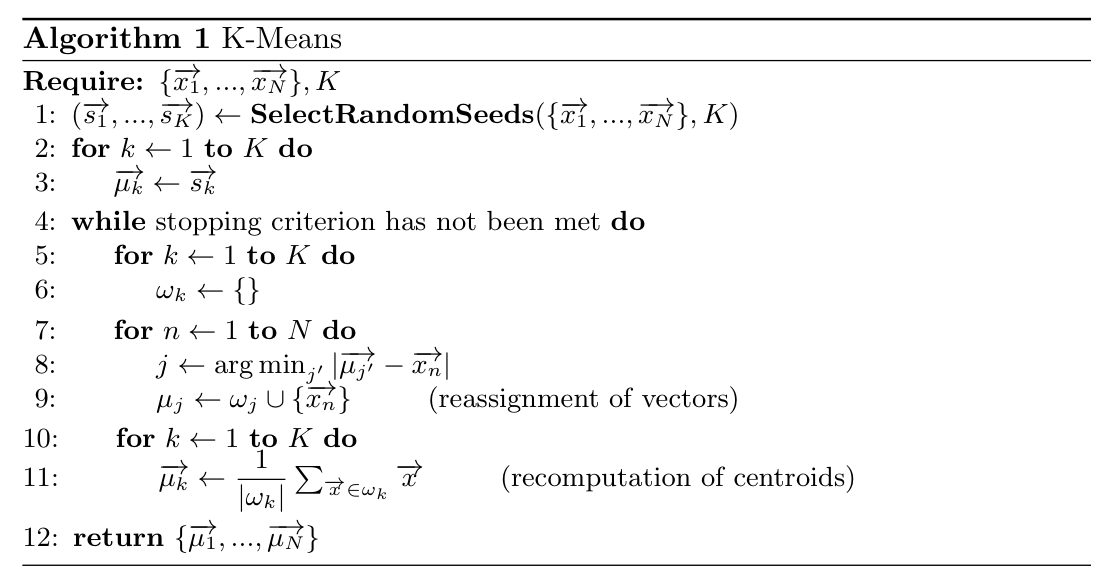
\includegraphics[width=10.5cm]{K-means.png}

	\framebreak
	
	\textcolor{white}{.}
	
	\vspace{0.5em}
	El primer paso de esta implementaci\'on de K-means es seleccionar al azar como centros iniciales de los cl\'usteres a K documentos, estas son las semillas. Luego, el algoritmo mueve los centros de los grupos en el espacio para minimizar el RSS. Este proceso se repite de manera iterativa hasta que se cumpla un criterio de parada.
	
	\vspace{1em}
	Criterios de parada:
	\begin{itemize}
		\item Cuando se ha completado un número fijo de iteraciones I. 
		\item Cuando la asignación de documentos a grupos no cambia entre iteraciones, excepto en los casos con un m\'inimo local malo.
		\item Cuando los centroides no cambian entre iteraciones.
		\item Cuando RSS cae por debajo de un umbral.
	\end{itemize}
}

	\subsection{Agrupamiento jer\'arquico}
	\frame
	{
		\frametitle{Agrupamiento jer\'arquico}
		El \textit{agrupamiento jerárquico} produce una jerarquía, una estructura que es más informativa que el conjunto no estructurado de clústeres devuelto por el agrupamiento particionado, no requiere que especifiquemos previamente el número de grupos y la mayoría son deterministas, sin embargo son m\'as ineficientes que los particionados. En una representación gráfica los elementos quedan anidados en jerarquías con forma de árbol.
		
		Los algoritmos de agrupamiento jerárquico pueden tener dos enfoques: de arriba hacia abajo (top-down) llamados de \textit{agrupamiento jer\'arquico aglomerativo} o de abajo hacia arriba (bottom-up) conocidos como de \textit{agrupamiento jer\'arquico divisivo}. 
	}
	
	
	\subsubsection{Agrupamiento jer\'arquico aglomerativo}
	\frame
	{
		\frametitle{Agrupamiento jer\'arquico aglomerativo}
		Los algoritmos de abajo hacia arriba tratan cada documento como un clúster único desde el principio y luego fusionan (o aglomeran) sucesivamente pares de grupos hasta que todos los grupos se han fusionado en uno solo que contiene todos los documentos. 
		Es por esto que se denomina agrupamiento jerárquico aglomerativo o HAC por sus siglas en ingl\'es. 
		
		Toman decisiones basadas en patrones locales sin tener inicialmente en cuenta la distribución global. Estas decisiones tempranas no se pueden deshacer.
	}

	\frame[allowframebreaks]
	{
		\frametitle{Medidas de similitud para cl\'usteres en HAC}
		
		\begin{itemize}
			\item \textbf{Agrupamiento por enlazamiento \'unico} (Single link clustering): La similitud entre dos cl\'usters es la similitud de los dos objetos más cercanos entre ellos (mayor similitud).
			
			\begin{center}
				$ sim(\omega_{i}, \omega_{j}) = max_{\overrightarrow{x} \in \omega_{i}, \overrightarrow{y} \in \omega_{j}} SIM(\overrightarrow{x}, \overrightarrow{y})$
			\end{center}
			
			\vspace{1em}
			\item \textbf{Agrupamiento por enlazamiento completo} (complete link clustering): La similitud entre dos cl\'usters es la similitud de los dos objetos más alejados entre ellos (menor similitud). 
			
			\begin{center}
				$ sim(\omega_{i}, \omega_{j}) = min_{\overrightarrow{x} \in \omega_{i}, \overrightarrow{y} \in \omega_{j}} SIM(\overrightarrow{x}, \overrightarrow{y})$
			\end{center}
			
			\vspace{1em}
			\item \textbf{Agrupamiento aglomerativo por promedio de grupo} (group-average agglomerative clustering): El agrupamiento aglomerativo por promedio de grupo o GAAC por sus siglas en ingl\'es, calcula la similitud promedio SIM-GA de todos los pares de documentos, incluidos los pares del mismo grupo (las auto-similitudes no están incluidas en el promedio).
			
			\begin{center}
				\footnotesize
				$ SIM-GA(\omega_{i}, \omega_{j}) = \dfrac{1}{(N_{i} + N_{j})(N_{i} + N_{j} - 1)} \sum_{\overrightarrow{x} \in \omega_{i} \cup \omega_{j}} \sum_{\overrightarrow{y} \in \omega_{i} \cup \omega_{j}, \overrightarrow{x} \neq \overrightarrow{y}} \overrightarrow{x} \cdot \overrightarrow{y} $
			\end{center}
			
			Este evalúa la calidad de un clúster basada en todas las similitudes entre documentos, evitando así castigar valores extremos como en los criterios de enlace único y enlace completo, que establecen la similitud del cl\'uster con la similitud de un solo par de documentos.
			
			\vspace{1em}
			\item \textbf{Agrupamiento por centroide} (centroid clustering): La similitud de dos cl\'usters est\'a definida como la similitud de sus centroides
			
			\begin{align}
				sim(\omega_{i}, \omega_{j}) &= \mu(\omega_{i})\cdot\mu(\omega_{j}) \nonumber\\
				&= \left(\dfrac{1}{N_{i}}\sum_{\overrightarrow{x} \in \omega_{i}}\overrightarrow{x}\right) \cdot \left(\dfrac{1}{N_{j}}\sum_{\overrightarrow{y} \in \omega_{i}}\overrightarrow{y}\right) \nonumber\\
				& = \dfrac{1}{N_{i}N_{j}} \sum_{\overrightarrow{x} \in \omega_{i}}\sum_{\overrightarrow{y} \in \omega_{j}}\overrightarrow{x}\cdot\overrightarrow{y} \nonumber
			\end{align}
			
			A diferencia de GAAC, el agrupamiento por centroide excluye el c\'alculo de pares del mismo cl\'uster.
		\end{itemize}
	
	}	
	
	\frame[allowframebreaks]
	{
		\frametitle{Algoritmo HAC}
		
		Dado un conjunto de N elementos a agrupar, el proceso básico del agrupamiento jerárquico es:
		\begin{enumerate}
			\item Se comienza con N cl\'usteres, resultado de asignar cada elemento al suyo propio. Se computa la matriz C de similitud de N×N.
			
			\item Se halla la similitud entre los pares de cl\'usteres con la medida deseada.
			
			\item Se toma el par más similar de clústeres y se combinan en un único clúster.
			
			\item Se calculan las similitudes entre el nuevo clúster y cada uno de los cl\'usteres antiguos.
			
			\item Se repiten los pasos 3 y 4 hasta que todos los elementos estén agrupados en un solo grupo de tamaño N.
		\end{enumerate}
	
	\framebreak
		\textcolor{white}{.}
	
	\vspace{0.9em}
	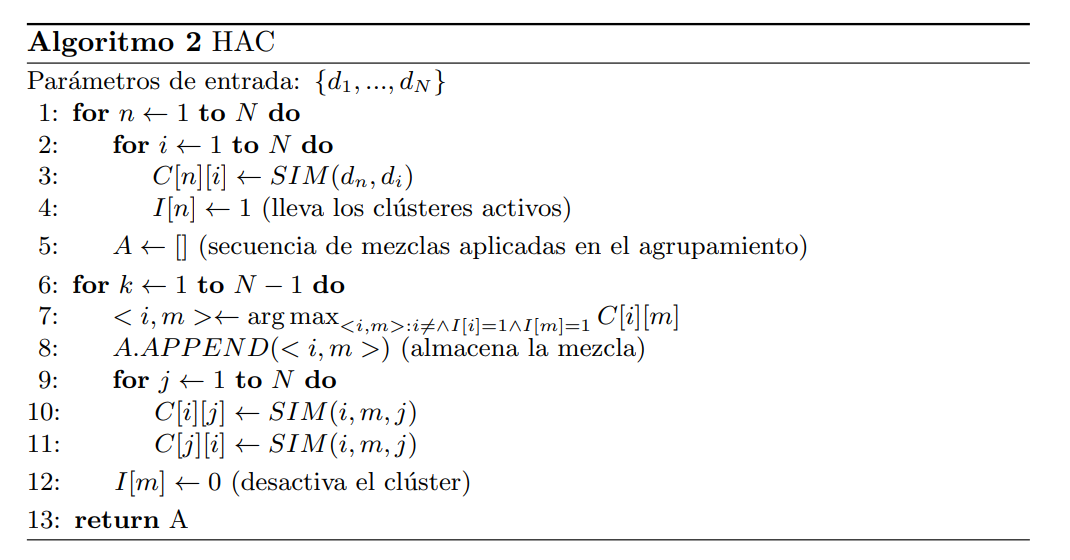
\includegraphics[width=10.5cm]{HAC.png}
	
	\framebreak
	Notas: 
	\begin{itemize}
		\item En cada iteración, los dos clústeres m\'as similares se fusionan y las filas y columnas del clúster fusionado i en C se actualizan.
		\item El agrupamiento se almacena como una lista de fusiones en A.
		\item I indica qué clústeres aún están disponibles para fusionarse. 
		\item La función SIM(i, m, j) calcula la similitud del grupo j con la fusión de los grupos i y M.
	\end{itemize}
	
	Una suposición fundamental en HAC es que la operación de fusión es mon\'otona, es decir si $ s_{1}, s_{2}, . . . , s_{K-1}$ son las similitudes de combinación de las fusiones sucesivas de un HAC, entonces se cumple $ s_{1} \geq s_{2} \geq . . . \geq s_{K-1}$.
	
	}	

	\subsubsection{Agrupamiento jer\'arquico divisivo}
	\frame
	{
		\frametitle{Agrupamiento jer\'arquico divisivo}
		Los algoritmos de arriba hacia abajo comienzan con todos los documentos en un grupo. El clúster se divide utilizando un algoritmo de agrupamiento particionado. Este procedimiento se aplica recursivamente hasta que cada documento está en su
		propio clúster.
		
		A pesar de necesitar un segundo algoritmo de agrupamiento particionado como una subrutina, tiene la ventaja de ser más eficiente si no generamos una jerarquía completa hasta las hojas de documentos individuales. Para un número fijo de niveles, y utilizando un algoritmo particionado eficiente como K-means, los algoritmos divisivos son lineales en el número de documentos y clústeres.
		
		Adem\'as se beneficia de la información completa sobre la distribución global al tomar decisiones de partición de alto nivel.
	}

	\subsection{Ventajas}
	\frame
	{
		\frametitle{Ventajas}
		\begin{itemize}
			\item No es necesario identificar las clases antes del procesamiento por lo que no se debe contar con expertos para este fin.
			
			\item Es útil para proporcionar estructura en grandes conjuntos de datos multivariados.
			
			\item Se ha descrito como una herramienta de descubrimiento porque tiene el potencial para revelar relaciones previamente no detectadas basadas en datos complejos.
			
			\item Debido a su amplia aplicación en dis\'imiles campos, cuenta el apoyo de una serie de paquetes de software, a menudo disponibles en la informática académica y otros entornos, por lo que se facilita su utilizaci\'on.
		\end{itemize}
	}

	\subsection{Desventajas}
	\frame
	{
		\frametitle{Desventajas}
		\begin{itemize}
			\item No se tiene una idea exacta de las clases creadas.
			\item No recibe retroalimentaci\'on.
		\end{itemize}
	}

	\subsection{Ejemplos de aplicaci\'on}
	\frame[allowframebreaks]
	{
		\frametitle{Ejemplos de aplicaci\'on}
		El agrupamiento es una técnica importante para descubrir subregiones o subespacios relativamente densos de una distribución de datos multidimensional. Se ha utilizado en la recuperación de información para muchos propósitos diferentes, como la expansión de consultas, la agrupación e indexación de documentos y la visualización de resultados de búsqueda. Permiten mejorar interfaz y experiencia de usuario y proporcionar una mayor eficacia o eficiencia del sistema de búsqueda. 
		
		\framebreak
		A continuaci\'on se describen con m\'as detalle algunas de las aplicaciones m\'as importantes:
		\begin{itemize}
			\item Agrupamiento de resultados de búsqueda (Search result clustering): La presentación predeterminada de los resultados de búsqueda (documentos devueltos en respuesta a una consulta) en la recuperación de información es una lista sencilla. Los usuarios escanean la lista de arriba a abajo hasta que encuentran la información que buscan. 
			
			En su lugar, en la agrupación en clústeres de resultados de búsqueda los documentos similares aparecen juntos, siendo más fácil escanear algunos grupos coherentes que muchos documentos individuales. Esto es particularmente útil si un término de búsqueda tiene diferentes significados.
			
			\item Dispersión-recopilación (Scatter-Gather): Su objetivo es tambi\'en una mejor interfaz de usuario. Este agrupa toda la colección para obtener grupos de documentos que el usuario puede seleccionar o reunir manualmente. Los grupos seleccionados se fusionan y el conjunto resultante se vuelve a agrupar. Este proceso se repite hasta que se encuentre un grupo de interés.
			
			La navegación basada en la agrupaci\'on de clústeres es una alternativa interesante a la búsqueda de palabras clave a la información estándar paradigma de recuperación de información. Esto es especialmente cierto en escenarios donde los usuarios prefieren navegar en lugar de buscar porque no están seguros de qué búsqueda términos a utilizar.
			
			\item Modelado de lenguaje (Language modeling): Explota directamente la hipótesis del agrupamiento para mejorar los resultados de búsqueda, basado en una agrupación de toda la colección. Usamos un índice invertido estándar para identificar un conjunto inicial de documentos que coincide con la consulta, pero luego agregamos otros documentos de los mismos grupos incluso si tienen poca similitud con la consulta. 
			
			Para evitar problemas de datos escasos en el modelado lenguaje enfocado a RI, el modelo de documento d se puede interpolar con un modelo de colección. Pero la colección contiene muchos documentos con términos atípicos de d. Al reemplazar el modelo de colección con un modelo derivado de grupo de d, obtenemos estimaciones más precisas de las probabilidades de ocurrencia de términos en d.
			
			\item Recuperaci\'on basada en cl\'usteres (Cluster-based retrieval): La agrupación también puede acelerar la búsqueda. 
			
			La búsqueda en el modelo de espacio vectorial equivale a encontrar los vecinos más cercanos a la consulta. El índice invertido admite la búsqueda rápida del vecino más cercano para la configuración estándar de RI. Sin embargo, a veces es posible que no podamos usar un índice invertido de manera eficiente. En tales casos, podríamos calcular la similitud de la consulta con cada documento, pero esto es lento. La hipótesis de agrupamiento ofrece una alternativa: encontrar los cl\'usteres que están más cerca de la consulta y sólo considerar los documentos de estos. Como hay muchos menos clústeres que documentos, se disminuye grandemente el espacio de b\'usqueda, y encontrar el clúster más cercano es rápido. Adem\'as los elementos que coinciden con una consulta son similares entre sí, por lo que tienden a estar en los mismos cl\'usteres, de esta forma la calidad no disminuye en gran medida.
		\end{itemize}
	}

	\section{Clasificaci\'on}
	\frame
	{
		\frametitle{Clasificaci\'on}
	}
	
	\subsection{Naive Bayes}
	\frame{
		\frametitle{Naive Bayes}
	}

	\subsection{Feature Selection}
	\frame{
		\frametitle{Feature Selection}
	}

	\subsection{K Nearest Neighbor}
	\frame{
		\frametitle{K Nearest Neighbor}
	}
	
	\subsection{Medidas de evaluaci\'on}
	\frame
	{
		\frametitle{Medidas de evaluaci\'on}	
	}
	
	\subsection{Ventajas}
	\frame
	{
		\frametitle{Ventajas}
	}
	
	\subsection{Desventajas}
	\frame
	{
		\frametitle{Desventajas}
	}
	
	\subsection{Aplicaciones en la Recuperaci\'on de la Informaci\'on}
	\frame
	{
		\frametitle{Aplicaciones en la Recuperaci\'on de la Informaci\'on}
	}
	
	\subsection{Otros ejemplos de aplicaci\'on}
	\frame
	{
		\frametitle{Otros ejemplos de aplicaci\'on}
	}

	\section{Conclusiones}
	\frame
	{
		\frametitle{Conclusiones}
	}

	\section{Referencias}
	\frame
	{
		\frametitle{Referencias}
	}
\end{document} 